\subsection{Composition, Inheritance, and Static Method Calls}
\textit{Show how to use a common piece of logic from two different classes, in three different ways: 1) by composition, 2) by inheritance, and 3) by static method calls, discuss the tradeoffs.}

\subsubsection{Inheritance}
The easiest way to think of class inheritance is that it is an "is-a" relationship. One class (child class) "is a" type of another class (super class).

For example, Cat and Dog classes are not the same, but they share common features. Both cats and dogs make a sound and they probably have a name. They have legs. We can abstract that common functionality into a super class called Animal.

\begin{figure}[H]\centering % Using \begin{figure*} makes the figure take up the entire width of the page
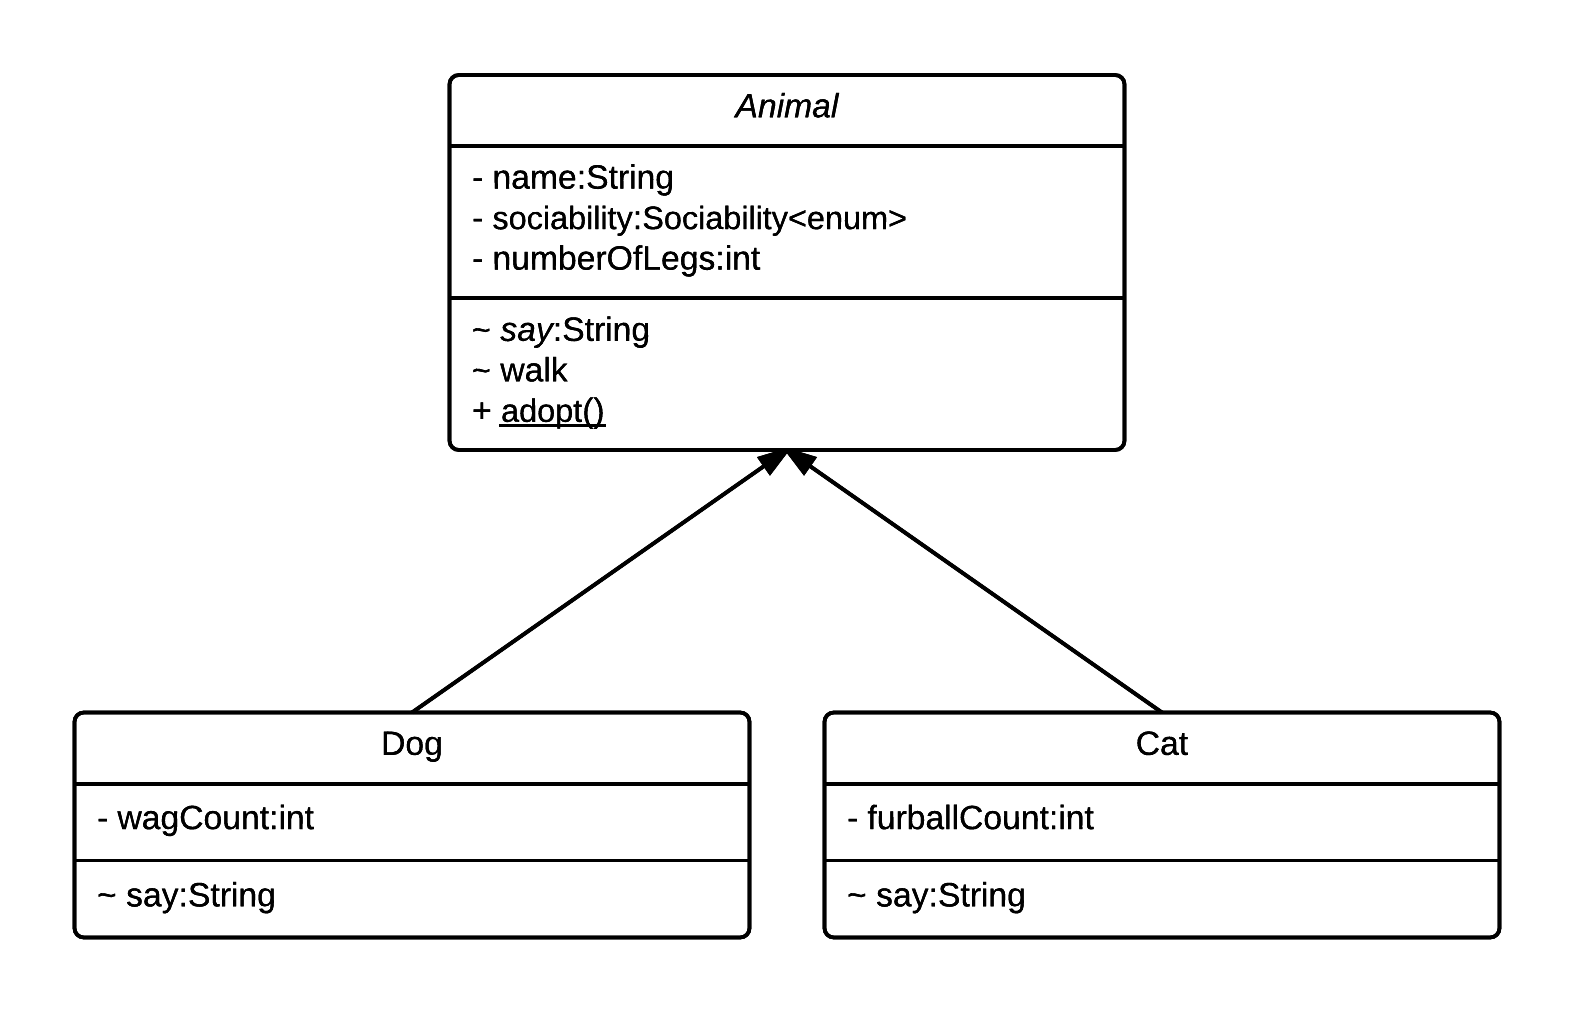
\includegraphics[width=0.9\linewidth]{images/inheritance}
\caption{Inheritance ("Is-a")}
\label{fig:inheritance}
\end{figure}

A Dog "is-a" Animal. The Cat "is-a" Animal. They inherit all package public, protected, and public methods and fields of Animal.

If the super class has any public or package public methods, the child classes can call them. For example, if Animal has a method walk:
\begin{lstlisting}[language=Java]

void walk() {
    String steps = this.getName() + " walks: ";
    for (int i = 0; i < numberOfLegs; i++) {
      steps += " step";
    }
    System.out.println(steps);
  }

\end{lstlisting}

We can call it from the Dog and Cat classes, as we did in the say method. There is no way to force Dog call the walk() method. If there is something that we want to enforce, there is a better way.

In Animal we have specified an abstract method say(). This way we force an Animal to have that functionality, but we let the child classes to specify what it means. 

\begin{lstlisting}[language=Java]
 public abstract String say();
\end{lstlisting}

Although they both say things, they say different things. Dogs bark and cats meow.
In order to do this, we also mark the Animal class abstract. That means that the user cannot create an instance of an Animal. We can only create instances of the child classes that are not abstract and implement the say method. This way we force the child classes to implement the say method.

Dog:
\begin{lstlisting}[language=Java]
// Dog:
@Override
  public String say() {
    String whatDoesTheCatSay = "Bark";
    for (int i = 0; i < wagCount; i++) {
      whatDoesTheCatSay += " (wag)";
    }
	super.walk();
    return whatDoesTheCatSay;
  }
  
// Cat:
@Override
  public String say() {
    String whatDoesTheCatSay = "Meouw";
    for (int i = 0; i < furballCount; i++) {
      whatDoesTheCatSay += " (cough)";
    }
    super.walk();
    return whatDoesTheCatSay;
  }
\end{lstlisting}

Cats and dogs also have unique features.  Cats have fur balls and dogs wag their tails. In the say method, we also add unique features. Dogs wag their tails and cats cough up furballs.

We can now create cats and dogs:
\begin{lstlisting}[language=Java]

Animal pluto = new Dog("Pluto", Animal.Sociability.VERY_SOCIAL, 3);
Animal sheba = new Cat("Sheba", 2);

// We can also create a Dog object
Dog pepper = new Dog("Pepper", Animal.Sociability.VERY_SOCIAL, 99);

\end{lstlisting}

The difference between pluto and pepper is that the pluto reference is of type Animal, and the pepper reference is of type Dog. There usually isn't a good reason to use the specific reference (pepper). It conceptually goes against the purpose of inheritance.

When we call the say method we have the following output:
\begin{lstlisting}[language=Java]
Bark (wag) (wag) (wag)

Person{pets=[{name:' Spot'}, {name:' Sheba'}]}
Sheba walks:  step step step step
Meouw (cough) (cough)
\end{lstlisting}

One of the benefits of inheritance is that we can treat Cat and Dog objects the same way, as instances of the Animal class. With that, we can, for example, store Cats and Dogs in the same collection:
\begin{lstlisting}[language=Java]
Animal sheba = new Cat("Sheba", 2);
Animal spot = new Dog("Spot", Animal.Sociability.VERY_SOCIAL, 5);
List<Animal> pets = new ArrayList<Animal>();
pets.add(spot);
pets.add(sheba);
\end{lstlisting}

See page \pageref{App:AppendixJInheritance} for full source code.

\subsubsection{Composition}

A composition is another way to share features between classes. The easiest way to think of it is a "has-a" relationship. For example, a Cat and a Dog "have-a" Tail.

\begin{lstlisting}[language=Java]
public class Tail {
  private boolean 	;
  private int length;

  public Tail(boolean docked, int length) {
    this.docked = docked;
    this.length = length;
  }
}
\end{lstlisting}

We can make the Animal class "have"a" tail. Because Dog "is-an" animal, it also "has-a" Tail. The same for the Cat.
\begin{figure}[H]\centering % Using \begin{figure*} makes the figure take up the entire width of the page
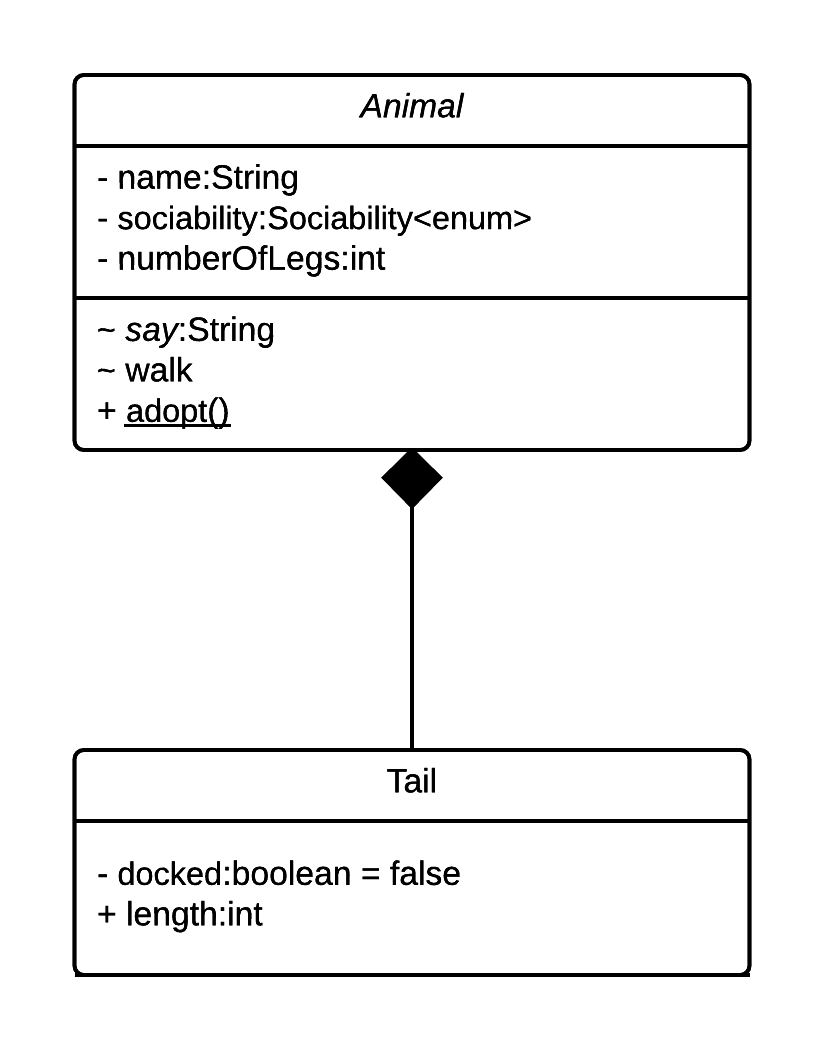
\includegraphics[width=0.9\linewidth]{images/composition}
\caption{Composition ("Has-A")}
\label{fig:composition}
\end{figure}

We just create a field in the Animal class for the tail.
\begin{lstlisting}[language=Java]
private Tail tail;
\end{lstlisting}

Now we can access it from Dog or Cat, as well as from Animal:
\begin{lstlisting}[language=Java]
super.setTail(tail);
\end{lstlisting}

See page \pageref{App:AppendixJComposition} for full source code.

\subsubsection{Static Methods}
There is yet another way to provide common functionality among several classes. We can declare a method or field static:

\begin{lstlisting}[language=Java]
public static String adopt(){
 return "Yay! Adopted Animal!";
}
\end{lstlisting}

The static keyword makes the class, field, or method special. We don't need to instantiate an object to access static members of a class. They are class-level parameters and fields:
\begin{lstlisting}[language=Java]
System.out.println(Animal.adopt());

// displays
Yay! Adopted Animal!
\end{lstlisting}
We can access the static adopt() method from the class, without using the new keyword to create an object.

A class might want to provide static fields, for example constants. In such case they should be also marked final, to avoid modification.

Also anything that we might want to share between objects of the same class should be marked static. For example, we might (for some strange reason) want to keep a count of instances of a class. If we declare a static field, all instances of the class will access exactly the same copy of that field. If one modifies it, it will be also show modified for the other instances.

See page \pageref{App:AppendixJTest} for full source code.